\section{Sicurezza nelle Reti di Calcolatori}

La sicurezza delle reti non è un singolo argomento, ma un insieme di proprietà che si desidera garantire. Le principali sono:
\begin{itemize}
    \item \textbf{Confidenzialità (Confidentiality):} Solo il mittente e il destinatario autorizzato possono comprendere il contenuto di un messaggio. Si ottiene tramite la \textit{crittografia}.
    \item \textbf{Integrità del Messaggio (Message Integrity):} Assicura che il messaggio non sia stato alterato (modificato, aggiunto o eliminato) durante il transito.
    \item \textbf{Autenticazione End-Point (End-point Authentication):} Permette a mittente e destinatario di confermare reciprocamente la propria identità.
    \item \textbf{Sicurezza Operativa (Operational Security):} Riguarda la protezione dell'infrastruttura di rete da attacchi, tramite strumenti come \textit{firewall} e \textit{Intrusion Detection Systems} (IDS).
\end{itemize}

\subsection{Princìpi di Crittografia}
La crittografia è la scienza di "scrivere in modo nascosto" e si basa su due componenti: un \textbf{algoritmo} (la ricetta) e una \textbf{chiave} (l'ingrediente segreto). Il messaggio originale è detto \textit{plaintext} (testo in chiaro) e il messaggio cifrato è detto \textit{ciphertext} (testo cifrato).

\subsubsection{Crittografia a Chiave Simmetrica}
In questo approccio, il mittente e il destinatario \textbf{condividono la stessa identica chiave segreta} (es. $K_S$).
\begin{itemize}
    \item \textbf{Funzionamento:} Alice cifra il messaggio $m$ usando la chiave $K_S$, ottenendo $K_S(m)$. Bob riceve $K_S(m)$ e usa la stessa chiave $K_S$ per decifrarlo e ottenere $m$.
    \item \textbf{Algoritmi Comuni:} \textbf{AES} (Advanced Encryption Standard) e \textbf{3DES} (Triple Data Encryption Standard). Questi sono \textit{cifrari a blocchi (block ciphers)}, che operano su blocchi di dati di dimensione fissa (es. 128 bit per AES).
    \item \textbf{Problema:} La \textbf{distribuzione della chiave}. Come fanno Alice e Bob a concordare la chiave segreta $K_S$ in modo sicuro, senza che un intruso (Trudy) possa intercettarla?.
\end{itemize}

\subsubsection{Crittografia a Chiave Pubblica}
Questo approccio, introdotto da Diffie e Hellman, risolve il problema della distribuzione delle chiavi usando una coppia di chiavi per ogni utente.
\begin{itemize}
    \item \textbf{Chiave Pubblica ($K_B^+$):} Nota a tutti nel mondo.
    \item \textbf{Chiave Privata ($K_B^-$):} Nota \textbf{solo} al proprietario (Bob).
\end{itemize}

\textbf{Funzionamento (Confidenzialità):}
\begin{enumerate}
    \item Se Alice vuole inviare un messaggio segreto a Bob, ottiene la chiave \textit{pubblica} di Bob, $K_B^+$.
    \item Alice cifra il messaggio $m$ usando la chiave pubblica di Bob: $c = K_B^+(m)$.
    \item Bob riceve $c$ e usa la sua chiave \textit{privata}, $K_B^-$, per decifrarlo: $m = K_B^-(c)$.
\end{enumerate}
Anche se Trudy intercetta $c$ e conosce $K_B^+$, non può decifrare il messaggio, perché solo $K_B^-$ (che solo Bob possiede) può farlo.

\begin{itemize}
    \item \textbf{Algoritmo Comune:} \textbf{RSA} (Rivest, Shamir, Adleman). Si basa sulla difficoltà computazionale di fattorizzare numeri molto grandi.
    \item \textbf{Uso Pratico (Session Key):} La crittografia a chiave pubblica è molto lenta (computazionalmente costosa). Nella pratica, si usa per scambiare in modo sicuro una \textbf{chiave di sessione} (una chiave simmetrica $K_S$ usa e getta). Il resto della comunicazione avviene poi velocemente usando la crittografia simmetrica con $K_S$.
\end{itemize}

\subsection{Integrità del Messaggio e Firme Digitali}
Come possiamo essere sicuri che un messaggio non sia stato modificato da Trudy?

\subsubsection{Funzioni di Hash Crittografiche}
Una \textbf{funzione di hash} (es. \textbf{MD5}, \textbf{SHA-1}, SHA-256) prende un messaggio $m$ di lunghezza arbitraria e produce un "impronta digitale" (fingerprint) a lunghezza fissa chiamata \textbf{hash} o \textit{message digest}, $H(m)$.

Proprietà crittografiche :
\begin{itemize}
    \item \textbf{A senso unico:} Dato $H(m)$, è impossibile risalire a $m$.
    \item \textbf{Resistenza alle collisioni:} È computazionalmente impossibile trovare due messaggi diversi $x$ e $y$ tali che $H(x) = H(y)$.
\end{itemize}

\subsubsection{Message Authentication Code (MAC)}
Un \textbf{MAC} (codice di autenticazione del messaggio) garantisce l'integrità del messaggio e l'autenticazione del mittente usando una \textit{chiave simmetrica segreta} $s$ (chiamata chiave di autenticazione) condivisa tra Alice e Bob.

\textbf{Funzionamento:}
\begin{enumerate}
    \item Alice calcola $h = H(m+s)$ (hash del messaggio concatenato con la chiave segreta $s$).
    \item Alice invia a Bob il pacchetto $(m, h)$. Questo $h$ è il MAC.
    \item Bob, che conosce $s$, riceve $(m, h)$ e calcola $H(m+s)$ in modo indipendente.
    \item Se il suo risultato corrisponde a $h$, Bob è sicuro che il messaggio proviene da Alice (perché solo lei conosce $s$) e che non è stato modificato (perché l'hash corrisponderebbe).
\end{itemize}
Il protocollo OSPF (discusso nel cap. 5) usa i MAC per autenticare i messaggi di routing.

\subsubsection{Firme Digitali}
Le \textbf{firme digitali} forniscono autenticazione e integrità del messaggio, ma usano la crittografia a \textit{chiave pubblica}. Hanno una proprietà fondamentale che i MAC non hanno: la \textbf{non ripudiabilità} (il mittente non può negare di aver inviato il messaggio).

\noindent\textbf{Funzionamento:}
\begin{enumerate}
    \item Alice calcola l'hash del messaggio, $H(m)$.
    \item Alice \textbf{cifra l'hash con la sua chiave privata}, $K_A^-(H(m))$. Questo risultato è la firma digitale.
    \item Alice invia a Bob il messaggio in chiaro e la firma: $(m, K_A^-(H(m)))$.
    \item Bob riceve il pacchetto.
    \item Bob calcola $H(m)$ per conto suo.
    \item Bob \textbf{decifra la firma usando la chiave pubblica di Alice}, $K_A^+(K_A^-(H(m)))$, ottenendo $H(m)'$.
    \item Se $H(m) = H(m)'$, il messaggio è autentico e integro. Bob è sicuro che provenga da Alice, perché solo la chiave privata di Alice poteva creare una firma che fosse decifrabile con la chiave pubblica di Alice.
\end{enumerate}

\subsubsection{Public Key Infrastructure (PKI) e Certification Authority (CA)}
C'è ancora un problema: come fa Alice a essere sicura che la chiave pubblica che sta usando sia davvero di Bob e non di Trudy?.

La soluzione è la \textbf{PKI (Infrastruttura a Chiave Pubblica)}.
Una \textbf{Certification Authority (CA)} (Autorità di Certificazione) è un'entità fidata (es. Verisign, Let's Encrypt) che si fa garante dell'identità delle persone/organizzazioni.
\begin{itemize}
    \item Bob porta la sua chiave pubblica $K_B^+$ alla CA.
    \item La CA verifica l'identità di Bob (es. tramite documenti).
    \item La CA usa la \textit{sua chiave privata} ($K_{CA}^-$) per creare un \textbf{certificato digitale}.
    \item Un certificato è un documento che dice: "Io, la CA, certifico che la chiave pubblica $K_B^+$ appartiene a Bob". Questo certificato è \textit{firmato digitalmente} dalla CA.
\end{itemize}
Ora, quando Bob vuole dimostrare chi è, invia ad Alice il suo certificato. Alice verifica la firma digitale della CA (usando la chiave pubblica della CA, che è pre-installata in tutti i browser) e, se la firma è valida, si fida del fatto che $K_B^+$ appartenga davvero a Bob.

\subsection{Autenticazione End-Point}
Come fa Bob (un server) a sapere che Alice (un client) è "live" (presente ora) e non è Trudy che sta semplicemente riproducendo un vecchio messaggio di Alice (attacco \textit{replay})?.

La soluzione è usare un \textbf{nonce}: un numero \textit{usato una sola volta} (Number used ONCE).

\noindent\textbf{Protocollo \textit{challenge-response} (ap4.0)}:
\begin{enumerate}
    \item Alice dice: "Sono Alice".
    \item Bob (il server) non si fida e le invia una "sfida": un numero casuale $R$ (il nonce).
    \item Alice deve \textit{provare} di essere Alice. Se condivide una chiave segreta $K_{A-B}$ con Bob, cifra il nonce e invia $K_{A-B}(R)$.
    \item Bob riceve la risposta, la decifra con $K_{A-B}$ e verifica che il risultato sia $R$.
\end{enumerate}
Dato che $R$ è stato generato pochi secondi fa, Bob sa che chi ha risposto è "live" (non è un replay) e conosce la chiave segreta (è Alice).

\subsection{TLS (Transport Layer Security) - Sicurezza a Livello Trasporto}
\textbf{TLS} (precedentemente noto come \textbf{SSL}) è il protocollo che fornisce sicurezza a \textbf{TCP}. È la "S" in \textbf{HTTPS}. Fornisce confidenzialità, integrità e autenticazione tra client e server.

\noindent \textbf{Fasi principali di TLS} :
\begin{enumerate}
    \item \textbf{Handshake TCP:} Viene stabilita una normale connessione TCP (handshake a 3 vie).
    \item \textbf{Handshake TLS (versione semplificata)}:
        \begin{itemize}
            \item Il client (browser) invia un "ClientHello" con un nonce ($R_{client}$) e la lista delle suite crittografiche che supporta.
            \item Il server (es. \texttt{google.com}) risponde con "ServerHello", la suite crittografica scelta, il suo \textbf{certificato} (contenente la sua chiave pubblica $K_S^+$) e un suo nonce ($R_{server}$).
            \item Il client \textit{verifica} il certificato del server (usando la chiave pubblica della CA). Ora è sicuro di parlare con \texttt{google.com} e non con Trudy.
            \item Il client genera un segreto, il \textbf{Pre-Master Secret (PMS)}, lo cifra con la chiave pubblica del server $K_S^+(PMS)$ e lo invia.
            \item Il server usa la sua chiave \textit{privata} $K_S^-$ per decifrare il PMS.
        \end{itemize}
    \item \textbf{Derivazione Chiavi:} Sia il client che il server usano i due nonce ($R_{client}, R_{server}$) e il PMS per generare (in modo indipendente ma identico) un set di chiavi di sessione simmetriche (es. una per cifrare i dati client->server, una per i dati server->client, e due per i MAC).
    \item \textbf{Trasferimento Dati Sicuro:} Da ora in poi, tutti i dati applicativi (es. richieste HTTP GET) vengono spezzettati in \textbf{record TLS}, cifrati con le chiavi di sessione simmetriche e autenticati con un MAC prima di essere inviati sulla connessione TCP.
\end{enumerate}

\subsection{IPsec - Sicurezza a Livello Rete}
\textbf{IPsec} è un protocollo che fornisce sicurezza a livello di rete (Livello 3). La sua applicazione più comune è la creazione di \textbf{VPN (Virtual Private Network)}.

A differenza di TLS (che protegge una singola applicazione), IPsec protegge \textit{tutti} i datagrammi IP che fluiscono tra due entità di rete (es. tra due router di sedi diverse, o tra un laptop di un dipendente e il router aziendale).

\noindent\textbf{Modalità Tunnel (Tunnel Mode):}
È la modalità usata per le VPN.
\begin{itemize}
    \item Il router della "Sede A" prende un intero datagramma IP (destinato alla rete interna della "Sede B"), lo tratta come un blocco di dati e lo \textbf{cifra} e \textbf{autentica} (usando il protocollo \textbf{ESP} - Encapsulation Security Payload).
    \item A questo pacchetto cifrato, il router aggiunge una \textbf{nuova intestazione IP} (in chiaro).
    \item L'indirizzo IP sorgente di questo nuovo header è il router della Sede A, e il destinatario è il router della Sede B.
    \item Il pacchetto viaggia su Internet. I router intermedi inoltrano il pacchetto basandosi sul nuovo header (in chiaro), ignari che il payload è un intero datagramma IP cifrato.
    \item Il router della "Sede B" riceve il pacchetto, rimuove l'header esterno, decifra il payload, ottiene il datagramma IP originale e lo inoltra all'host corretto nella sua rete interna.
\end{itemize}

\begin{center}
    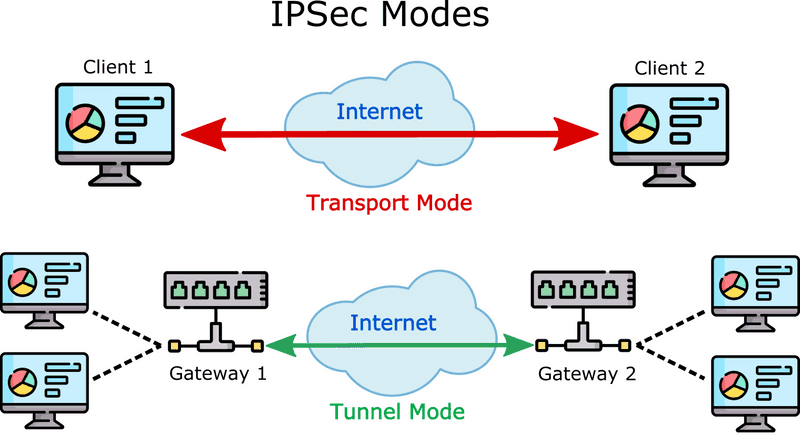
\includegraphics[width=0.9\textwidth]{img/ipsec_tunnel_mode.png}
\end{center}

\noindent\textbf{Security Association (SA):}
Prima di poter inviare dati, i due router (Sede A e Sede B) devono negoziare i parametri di sicurezza. Creano una connessione logica chiamata \textbf{Security Association (SA)}.
Una SA è unidirezionale e definisce:
\begin{itemize}
    \item L'algoritmo di crittografia (es. AES) e la chiave simmetrica da usare.
    \item L'algoritmo di integrità (es. HMAC-SHA) e la chiave MAC da usare.
\end{itemize}
Per una comunicazione bidirezionale servono due SA. La negoziazione automatica di queste SA avviene tramite il protocollo \textbf{IKE (Internet Key Exchange)}.

\subsection{Sicurezza Operativa: Firewall e IDS}
Oltre a cifrare i dati, le reti si proteggono usando difese perimetrali.

\subsubsection{Firewall}
Un \textbf{firewall} è un dispositivo hardware o software posto tra la rete interna di un'organizzazione e la Internet pubblica. Ispeziona tutto il traffico in entrata e in uscita e decide se bloccarlo o permetterlo, in base a un set di regole (policy).

Tipi di firewall :
\begin{itemize}
    \item \textbf{Packet Filter (Filtro di Pacchetti Tradizionale):} Prende decisioni basandosi solo sugli header IP e TCP/UDP (indirizzi IP, numeri di porta, flag TCP come SYN/ACK). È veloce ma "stupido". Ad esempio, una regola può bloccare tutto il traffico in entrata tranne quello destinato alla porta 80 (Web server).
    \item \textbf{Stateful Filter (Filtro Stateful):} Un firewall più intelligente. Oltre a controllare gli header, \textbf{tiene traccia delle connessioni TCP attive} (usando una "tabella delle connessioni"). Permette l'ingresso di un pacchetto di risposta dall'esterno solo se appartiene a una connessione \textit{già iniziata dall'interno}.
    \item \textbf{Application Gateway (Proxy):} Il firewall più avanzato e lento. Agisce come intermediario per un'applicazione specifica (es. un proxy HTTP). L'utente interno si connette al proxy, e il proxy si connette al server esterno per conto dell'utente. Questo permette un'ispezione profonda del contenuto (Deep Packet Inspection) e un controllo a livello utente (es. "Alice può telnet, Bob no").
\end{itemize}

\subsubsection{Intrusion Detection Systems (IDS)}
Un \textbf{IDS} è un dispositivo che monitora la rete alla ricerca di attività sospette o malevole e, se le rileva, genera un \textbf{allarme} (alert) per l'amministratore di rete. Un \textbf{IPS} (Intrusion Prevention System) è un IDS che può anche \textit{bloccare} attivamente il traffico sospetto.

Tipi di IDS :
\begin{itemize}
    \item \textbf{Signature-based IDS (Basato su firme):} Funziona come un antivirus. Ha un database di "firme" (pattern) di attacchi noti (es. un certo pattern di bit nel payload che corrisponde a un worm, o una scansione di porte). Se un pacchetto corrisponde a una firma, scatta l'allarme. È efficace contro attacchi noti, ma inutile contro attacchi nuovi ("zero-day").
    \item \textbf{Anomaly-based IDS (Basato su anomalie):} L'IDS prima "impara" come appare il traffico di rete "normale" (crea un profilo statistico). Successivamente, segnala qualsiasi traffico che devia significativamente da questa norma (es. un flusso ICMP improvviso, un host interno che contatta migliaia di IP esterni). Può rilevare attacchi nuovi, ma è soggetto a molti "falsi positivi".
\end{itemize}


